\chapter{Diseño}

En este capítulo se describirá el diseño de esta aplicación para poder llevar acabo este flujo. A muy alto nivel, el flujo de la aplicación es el siguiente:

\begin{enumerate}
    \item El usuario introduce un mensaje.
    \item El cliente envía el mensaje al chatbot.
    \item \label{itm:paso-respuesta} El chatbot recibe el mensaje del usuario e inicia un proceso de formulación de la respuesta basada en la \textbf{intención} y las \textbf{entidades} semánticas del mensaje.
    \item El chatbot envía la respuesta al usuario.
\end{enumerate}

Cabe mencionar que cada mensaje enviado no requiere de un estado ni una sesión, por lo que el diseño de esta aplicación con el flujo descrito asume que \textbf{únicamente el mensaje contiene la información necesaria para poder responderlo.}

\section{Arquitectura de la Aplicación}

El desarrollo de esta aplicación requiere de los siguientes componentes:

\begin{figure}[ht]
    \centering
    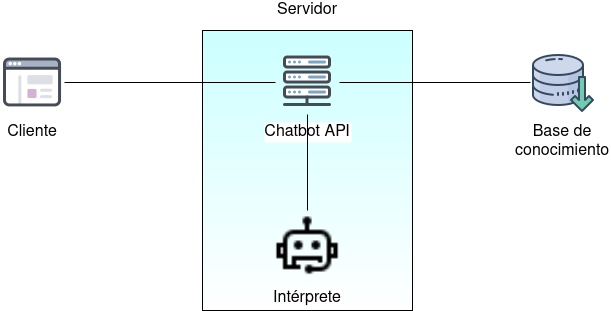
\includegraphics[scale=0.6]{images/5/arquitectura-general.png}
    \caption{Arquitectura de los componentes del sistema.}
    \label{fig:arquitectura-general}
\end{figure}

\begin{itemize}
    \item \textbf{Cliente}: Es la herramienta que solicita los servicios, utilizada por un usuario para poder enviar un mensaje mediante el chat.
    \item \textbf{Chatbot API}: Es la puerta de enlace al API del chatbot. Recibe peticiones HTTP que contienen un mensaje y devuelve una respuesta para el chat del cliente.
    \item \textbf{Intérprete}: Componente de procesamiento de lenguaje natural que procesa la interpretación del mensaje y construcción de las respuestas.
    \item \textbf{Base de Conocimiento}: Base de datos con los documentos normativos y la representación semántica de los mismos utilizada por el Intérprete.
\end{itemize}

\section{Fases del diseño}

Para desarrollar la aplicación, se requiere las siguientes fases de diseño:

\begin{enumerate}
    \item Diseño de la base de Conocimiento
    \item Diseño del chatbot
    \item Diseño del sistema cliente
\end{enumerate}

% Adicionalmente, se agrega un apartado adicional para detallar los aspectios del \textit{diseño de la conversación}.


%
%
%   DISEÑO DE LA BASE DE CONOCIMIENTO
%
%


\section{Diseño de la Base de Conocimiento}

En esta fase se pretende modelar el conocimiento y su proceso de estructuración a un formato que el chatbot usará para responder preguntas.

\subsection{Modelo de datos}

\begin{figure}[ht]
    \centering
    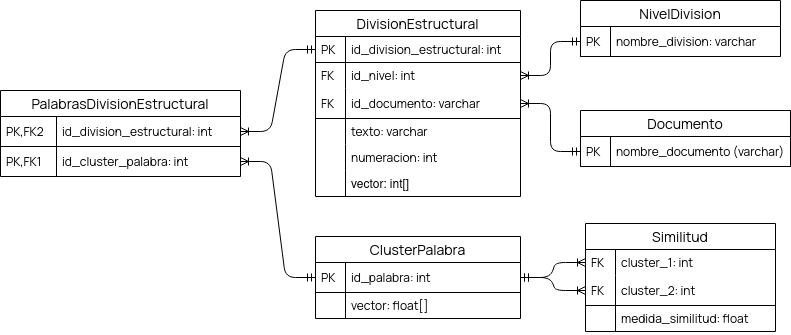
\includegraphics[scale=0.55]{images/5/diagrama-relacional.png}
    \caption{Modelo Relacional.}
    \label{fig:diagrama-relacional}
\end{figure}

Con este modelo se pretende persistir los elementos de los documentos normativos, así como una representación necesaria para que el intérprete pueda procesarlos.

\begin{enumerate}
    \item \textbf{NivelDivision}: Catálogo de los elementos de la división estructural de la ley definidos en el requisito funcional \ref{itm:consultar-reglamento}.
    
    \begin{itemize}
        \item \textbf{nombre\_division}: llave primaria, identifica al nivel en las categorías de \textit{título}, \textit{capítulo}, \textit{sección} o \textit{artículo}.
    \end{itemize}
    
   \item \textbf{Documento}: Son los documentos que contienen los reglamentos del Instituto Politécnico Nacional. Su función es recopilar los reglamentos.
   
   \begin{itemize}
        \item \textbf{nombre\_documento}: llave primaria, nombre que identifica al documento normativo (e.g. \textit{Reglamento Interno del Instituto Politécnico Nacional}).
    \end{itemize}
   
   \item \textbf{DivisionEstructural}: Segmento estructural de los documentos legales. Contienen el texto como tal de los reglamentos:
   
   \begin{itemize}
        \item \textbf{id\_division\_estructural}: llave primaria, es el identificador único del reglamento.
        \item \textbf{id\_nivel}: llave foránea, referencia a la tabla \textbf{Nivel}.
        \item \textbf{id\_documento}: llave foránea, referencia a la tabla \textbf{Documento}.
        \item \textbf{texto}: Contenido textual del reglamento.
        \item \textbf{numeracion}: la enumeración del elemento correspondiente a su nivel (e.g., titulo \textit{1}, artículo \textit{25}, sección \textit{2})
        \item \textbf{vector}: Representación del texto en vector binario que codifica el conocimiento. Su uso se explicó en la sección \ref{sec:deteccion-parafrasis}. 
    \end{itemize}
   
   \item \textbf{PalabraCluster}: Tabla que contiene la representación vectorial de un conjunto de palabras del vocabulario. Su propósito se definió en la sección. \ref{subsec:reduccion-vocabulario}.
   
   
   \begin{itemize}
       \item \textbf{id\_cluster}: llave primaria, identificador del cluster y \textit{también funciona como índice del vector (vector unitario)} para su vector unitario.
       \item \textbf{palabra}: cadena de texto representando a la palabra del vocabulario.
   \end{itemize}
   
   \item \textbf{Similitud}: Tabla representando la similitud entre dos palabras, cuya llave primaria se constituye de las llaves foráneas de ambas palabras:
   
   \begin{itemize}
       \item \textbf{palabra\_1}: llave foránea, referencia a la a tabla \textbf{PalabraCluster}.
       \item \textbf{palabra\_2}: llave foránea, referencia a la a tabla \textbf{PalabraCluster}.
       \item \textbf{medida\_similitud}: similitud cuantificada de acuerdo a un modelo lingüístico utilizando un espacio vectorial entrenado previamente.
   \end{itemize}

    \item \textbf{PalabrasDivisionEstructural}: Relación de muchos a muchos de las tablas \textbf{DivisionEstructural} y \textbf{ClusterPalabra}. Su propósito es agrupar las palabras existentes en el texto para agilizar la construcción del vector binario.
\end{enumerate}

\subsection{Diagrama de Actividad: Transformación y Carga de Documentos Normativos}

\begin{figure}[ht]
    \centering
    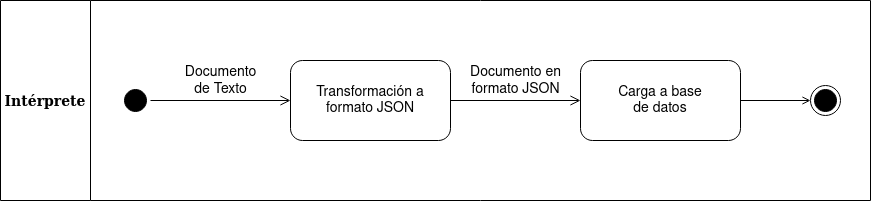
\includegraphics[scale=0.54]{images/5/actividad-transformacion.png}
    \caption{Proceso de transformación y carga de reglamentos estructurados.}
    \label{fig:actividad-transformacion}
\end{figure}

En este proceso, se transforma de manera uniforme a documentos del marco normativo en una estructura útil para el chatbot. Se elige un formato TXT semi-estructurado que separdo por líneas de salto cada título, capítulo, sección y artículo. Este se transforma a un archivo JSON con estructura jerárquica por la naturaleza de los reglamentos. Esto ayuda a revisar también la consistencia del archivo de texto.

\begin{enumerate}
    \item \textbf{Transformación a formato JSON}: Recibe como entrada un archivo semi-estructurado y produce un archivo en formato JSON con la siguiente estructura:
    
    \begin{itemize}
        \item \textbf{items}: arreglo de objetos con los siguientes atributos:
        
        \begin{itemize}
            \item \textbf{contenido}: objeto anidado recursivo
            \item \textbf{enumeracion}: número de elemento de la división estructural
            \item \textbf{texto}: contenido textual del elemento
        \end{itemize}
        
        \item \textbf{nivel}: nombre del nivel de la división estructural
    \end{itemize}
    
    \item \textbf{Carga a base de datos}: Se recibe como entrada el archivo JSON estructurado jerŕquicamente y se recorre en forma de árbol a todos sus elementos para posteriormente cargarlo en la tabla \textbf{DivisionEstructura} del modelo de datos.
\end{enumerate}


%
%
%   DISEÑO DEL CHATBOT
%
%


\section{Diseño del Chatbot}

\subsection{Diseño del Algoritmo de Detección de Paráfrasis}

La medida de similitud de palabras requiere de una representación de word embedding sobre un espacio vectorial, que se obtiene mediante métodos de aprendizaje automático utilizando redes neuronales. Cabe mencionar que \textbf{la construcción del modelo para representar palabras de esta manera está fuera del alcance de este proyecto}.

La consulta introducida será de la siguiente forma:

\begin{itemize}
    \item ¿Cuáles artículos hablan acerca de la \underline{baja temporal del semestre}?
    \item ¿Me puedes decir cuáles reglamentos hablan sobre \underline{rayar o dañar propiedad de la escuela}?
\end{itemize}

El segmento subrayado será nuestra oración de interés y deberá estar sujeto a los requisitos mencionados para la preparación de los datos. Posteriormente, se ejecutará lo siguiente:

\begin{enumerate}
    \item Se quitan palabras irrelevantes que forman parte de
    \item Se quitan las palabras vacías de la consulta y las resultantes se llevarán a su forma lematizada.
    \item Se construye el vector de consulta $q$: se establece un valor de 1 en todos los índices del vector cuya dimensión pertenece a una palabra presente en la consulta, de lo contrario se establece en 0 (i.e., es la suma de los vectores unitarios de las palabras que aparecen en la consulta.)
    \item Se iterarán sobre todos los artículos $a$ de un reglamento y se ejecutará la función de similitud entre el vector de consulta mediante $sim(q, a)$.
    \item Se ordenarán conforme al resultado de relevancia obtenido por la función de similitud y se obtendrán todos aquellos que superen un umbral $sim(q, a)  > 0.7$.
    \item Se devuelve como salida del algoritmo la lista de artículos que cumplen la condición anterior.
\end{enumerate}

\begin{figure}
    \begin{algorithm}[H]
        \SetAlgoLined
        \SetKwInput{Entrada}{Entrada}
        \SetKwInput{Salida}{Salida}
        \SetKwFor{ParaCada}{ParaCada}{hacer}{fin para cada}
        \SetKwIF{SSi}{EnOtroCasoSi}{EnOtroCaso}{si}{entonces}{sin ́o, si}{sin ́o}{fin si}

        \Entrada{Cadena de texto $q$ con la consulta del usuario.}
        \Salida{Lista de artículos $a$ relevantes a la consulta.}
        
        $q_{norm}$ = quitar\_palabras\_vacias($q_entrada$)\;
        $q_w$ = lematizar($q_{norm}$)\;
        $q_v$ = vectorizar($q_w$)
        umbral\_aceptable\_similitud = 0.7\;
        articulos\_relevantes = inicializar\_lista\_vacia()\;
        \ParaCada{articulo  $a$ en la base de conocimiento}{
            $a_v$ = vectorizar($a$)\;
            nivel\_parafrasis = calcular\_similitud($q_v$, $a_v$)\;
            \SSi{nivel\_parafrasis $\geq$ umbral\_aceptable\_similitud}{
                agregar(articulos\_relevantes, $a$)\;
            }
        }
        \caption{Algoritmo de detección de paráfrasis.}
    \end{algorithm}
    \label{fig:algoritmo-deteccion-parafrasis}
\end{figure}

\newpage

\subsection{Diagrama de Secuencia: Interacción Usuario-Chatbot}

En la figura \ref{fig:secuencia-general} se muestra el diagrama de secuencia, el cual contiene un bloque denominado \textbf{Formular respuesta}. Este bloque se ejecutará de acuerdo a las intenciones detectadas y que se describieron en en el requisito funcional \ref{itm:requisito-intenciones}.


Cabe mencionar que la intención \textit{Buscar conceptos} es el que ejecutará el algoritmo descrito en la figura \ref{fig:algoritmo-deteccion-parafrasis}.

\begin{figure}[ht]
    \centering
    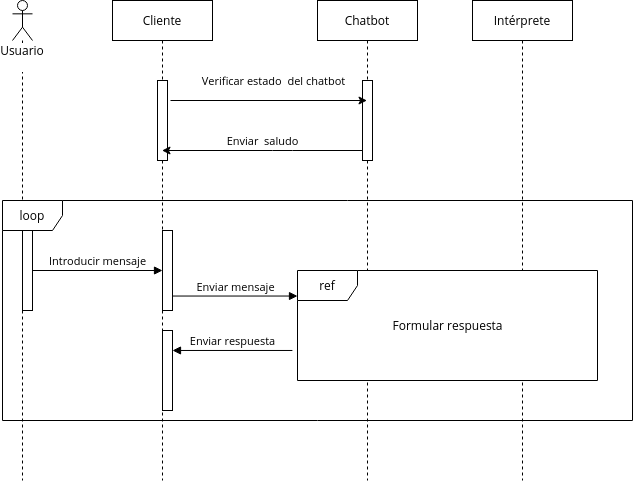
\includegraphics[scale=0.7]{images/5/diagrama-secuencia.png}
    \caption{Diagrama de la secuencia Interacción Usuario-Chatbot.}
    \label{fig:secuencia-general}
\end{figure}

\newpage

\subsection{Diagrama de Actividad: Reducir Vocabulario}
\label{subsec:reduccion-vocabulario}

El español tiene 88,000 palabras en su diccionario. Cargar en memoria todas las palabras y calcular una matriz de similitud $M_{88000,88000}$ requiere de 7,744,000,000 operaciones con sus respectivas asignaciones de memoria, que podría requerir hasta 1 TB de memoria.

Es por esto que se buscará reducir los vectores de palabras reduciéndolos a \textbf{clusters} de palabras, que realmente es reducir un grupo de vectores al promediarlos dando por resultado un centro de esa agrupación que se vuelve el nuevo vector de palabra.

La agrupación de estos vectores de palabras son \textit{semánticamente similares}, por lo que deberían significar lo mismo o algo parecido. Entonces se buscará reducir la cantidad de vectores para optimizar procesamiento y almacenamiento, pero la cantidad reducida no debe afectar \textit{la distribución de vectores para no perder su valor semántico}.

\begin{figure}[ht]
    \centering
    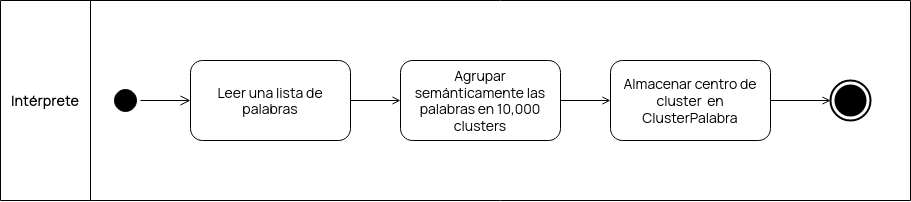
\includegraphics[scale=0.5]{images/5/actividad-reducir-vocabulario}
    \caption{Diagrama de la actividad: Reducir vocabulario.}
    \label{fig:reducir-vocabulario}
\end{figure}

La figura \ref{fig:reducir-vocabulario} describe el proceso a un nivel general. En esta actividad se detalla la reducción del vocabulario, promediando las representaciones vectoriales en agrupaciones utilizando el algoritmo K-Means.

\begin{enumerate}
    \item \textbf{Leer lista de palabras}: Se lee un archivo de texto con el vocabulario de entrenamiento con palabras en español.
    \item \textbf{Agrupar semánticamente las palabras en 10,000 clusters}: Se agrupan las palabras en 10,000 clusters utilizando la similitud de palabras cono medida de distancia.
    \item \textbf{Almacenar centro de cluster en ClusterPalabra}: El resultado de las agrupaciones se almacenan en la tabla \textbf{ClusterPalabra}.
\end{enumerate}

\subsection{Diagrama de Actividad: Inicialización}

\begin{figure}[ht]
    \centering
    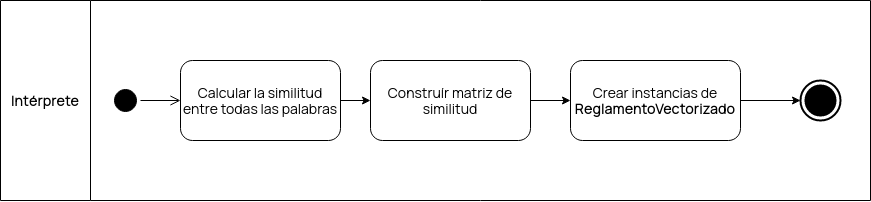
\includegraphics[scale=0.5]{images/5/actividad-inicializacion}
    \caption{Diagrama de la actividad: Inicialización de matriz de similitud y vector de palabras.}
    \label{fig:actividad-inicializacion}
\end{figure}

Antes de que el servicio del chatbot se encuentre funcional, la primera actividad que debe ejecutarse es la de inicialización del modelo utilizado en el algoritmo \ref{fig:algoritmo-deteccion-parafrasis} (la matriz $\mathbf{W}$). La similitud calculada se almacena en la tabla \textbf{Similitud} de la figura \ref{fig:diagrama-relacional} para posteriormente poblar la matriz.

Los pasos de esta actividad son:

\begin{enumerate}
    \item \textbf{Calcular la similitud entre todas las palabras}: Utilizando un modelo de espacio vectorial, iterar sobre todos las instancias de \textbf{ClusterPalabra} y calcular su similitud con todos las otras instancias de \textbf{ClusterPalabra}, incluso consigo mismo.
    \item \textbf{Construir matriz de Similitud}: Los elementos de la matriz se llenarán como se especifica en la sección \ref{fig:algoritmo-deteccion-parafrasis}; es decir, el índice del renglón y la columna será \textbf{id\_palabra} por lo que la dimensión de los vectores y la cantidad de columnas y renglones de $\mathbf{W}$ son la cantidad de instancias en \textbf{ClusterPalabra}.
    \item \textbf{Poblar tabla ReglamentoVectorizado}: Representar cada elemento de la tabla \textbf{DivisiónEstructural} que sea artículo en su representación binaria; por cada palabra que aparezca en su texto, obtener su \textbf{ClusterPalabra} a la que pertenece y establecer un valor de 1 en el índice indicado por el identificador de \textbf{ClusterPalabra}.
\end{enumerate}



\subsection{Diagrama de Actividad: Formular respuesta}

Esta actividad es el detalle de lo que ocurre cuando se requiere atender un mensaje de un usuario, especificado en el diagrama de secuencia del proceso general de la aplicación en la figura \ref{itm:requisito-intenciones}. El proceso se desribe de la siguiente manera:

\begin{enumerate}
    \item \textbf{Recibe mensaje}: Se recibe la cadena de texto que introduce el usuario a través del cliente.
    \item \textbf{Reconocer intención}: La cadena de texto se introduce a un clasificador de intenciónes que categoriza la intención en una de las siguientes: {\textit{saludar}, \textit{despedir}, \textit{solicitar\_reglamento}, \textit{buscar\_conceptos}}.
    \item \textbf{Se evalúa la intención y se elige una acción}
    
    \begin{enumerate}
        \item La intención es \textit{saludar}: Se elige un mensaje del catálogo de saludos de acuerdo a la hora del día y se informa acerca del uso de la aplicación (i.e., que cosas puede hacer y ejemplos de mensajes).
        \item La intención es \textit{despedir}: Se elige un mensaje del catálogo de despedidas.
        \item La intención es \textit{solicitar\_reglamento}: 
        
        \begin{enumerate}
            \item \textbf{Extraer entidades: nivel de reglamento y número}: Del mensaje del usuario se reconoce y se extraen la entidades \textbf{nivel}, que representa el nivel de división estructural, y \textbf{número} que representa la enumeración en el documento normativo.
            \item \textbf{Recuperar reglamento}: utilizando el \textbf{nivel} y \textbf{enumeración}
        \end{enumerate}
        
        \item La intención es \textit{buscar\_conceptos}: Se ejecuta lo siguiente
        
        \begin{enumerate}
            \item \textbf{Extraer enunciado}: se elimina la parte solicitante (\textit{qué artículos hablan acerca de..., en dónde dice que...}) del mensaje y se regresa única mente el texto con los conceptos relevantes, el cual es básicamente el restod e la oración
            \item \textbf{Ejecutar algoritmo de similitud de conceptos sobre todos los artículos}: Iterar sobre todos los elementos de \textbf{ReglamentoVectorizado} y regresar una lista de todos los \textbf{artículos} vector tenga una similitud por encima del 0.5.
            \item \textbf{Recuperar artículos}: Recuperar cada \textbf{artículo} de los documentos normativos y regresar un mensaje con la lista de artículos recuperados.
        \end{enumerate}
        
        \item La intención es \textit{desconocida}: Se regresa un mensaje al usuario indicando que no se reconoce lo que quiere hacer, agregando información acerca de lo que el chatbot puede hacer.
    \end{enumerate}
    
    \item La intención es \textit{desconocida}: Esto ocurre cuando no se entiende lo que el usuario quiere. Se regresa un mensaje informativo al usuario indicando de las funciones que hace el chatbot.
    
    \item \textbf{Devolver respuesta}: El mensaje construido se devuelve al cliente que solicitó el servicio del chatbot.
\end{enumerate}

\newpage

\begin{figure}[ht]
    \centering
    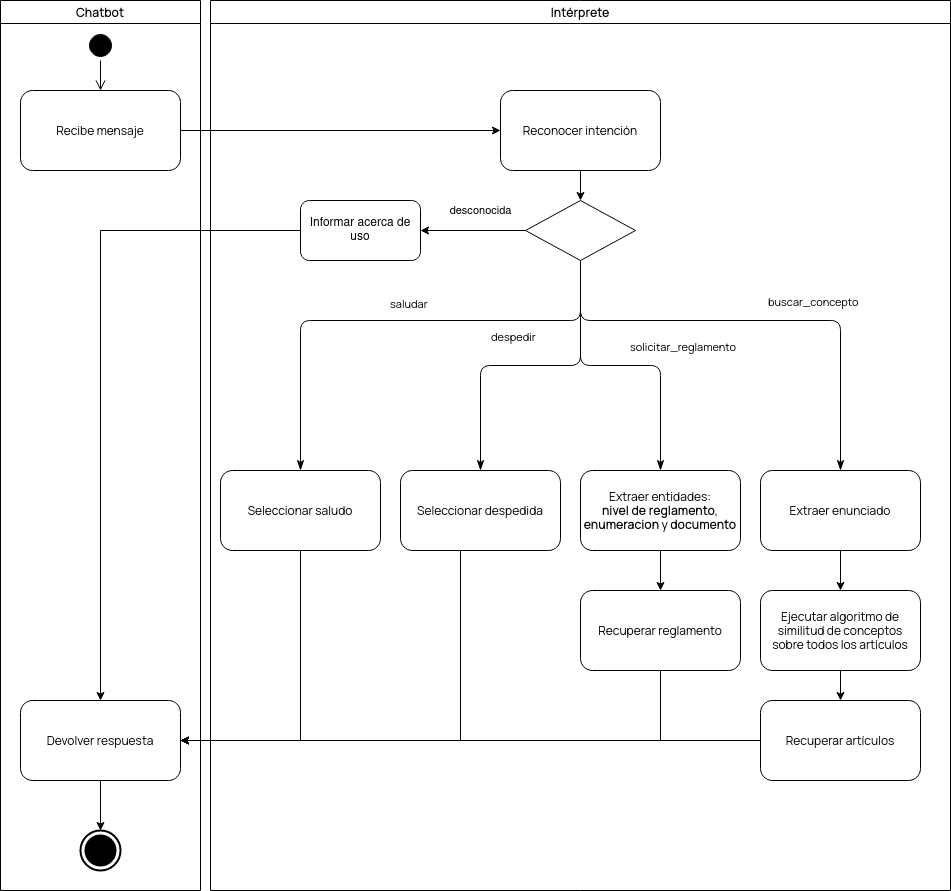
\includegraphics[scale=0.49]{images/5/diagrama-actividades}
    \caption{Diagrama de la actividad: Formular Respuesta.}
    \label{fig:actividad-responder}
\end{figure}


%
%
%   DISEÑO DE LA INTERFAZ DE USUARIO
%
%

\newpage

\section{Diseño del Sistema Cliente}

\subsection{Casos de Uso}

\begin{figure}[ht]
    \centering
    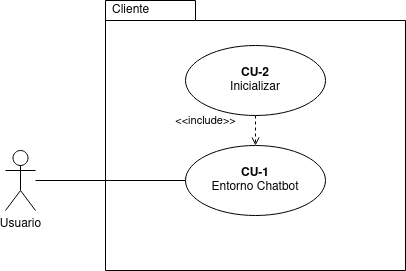
\includegraphics[scale=0.61]{images/5/casos-de-uso}
    \caption{Representación del caso de uso del usuario mediante el cliente.}
    \label{fig:diagrama-casos-de-uso} 
\end{figure}

\subsubsection{Actores}

Debido a que este sistema proporciona un chatbot disponible para el público de la comunidad de ESCOM, se define solo un actor que realiza una interacción con el sistema:

\begin{itemize}
    \item \textbf{Usuario}: Es todo aquel que usa el sistema que usa el sistema como herramienta auxiliar para la asesoría. Obtiene su utilidad al utilizar el sistema cliente enviando mensajes de texto al chatbot.
\end{itemize}

\subsection{Descripción de los casos de uso}

% Listado de casos de uso
\noindent\makebox[\linewidth]{\rule{\textwidth}{0.4pt}}
\begin{enumerate}[leftmargin=2.5cm ,label={\bfseries CU-\arabic*}]
    
    % Inicia CU
    \item \textbf{Entorno Chatbot}: 
    
        \textbf{Descripción}: Permite la interacción entre el usuario y el chatbot para enviar mensaje.
        
        \textbf{Pre-condiciones}: 
        
        \begin{itemize}
            \item Debe haber una conexión con el servidor
        \end{itemize}
        
        \textbf{Post-condiciones}: 
        
        \begin{itemize}
            \item No existe post-condición.
        \end{itemize}
        
        \textbf{Errores}: 
        
        \begin{itemize}
            \item No se puede acceder al servidor.
        \end{itemize}
        
        \textbf{Flujo}:
        
        \begin{enumerate}[label=\arabic*)]
            \item El Usuario escribe mensaje.
            \item El Usuario envía mensaje al servidor.
            \item El Usuario espera respuesta del chatbot.
            \item Trayectoria alternativa A:

                \begin{itemize}
                    \item El cliente recibe respuesta del chatbot.
                    \item El cliente muestra el mensaje de respuesta al mensaje del usuario.
                \end{itemize}

            \item Trayectoria alternativa B:

                \begin{itemize}
                    \item El cliente no puede acceder al servidor.
                    \item El cliente muestra un mensaje en el \textbf{Área de Diálogo} diciendo: "No se pudo conectar con el chatbot. Intente de nuevo mas tarde."
                \end{itemize}
            \item Continúa en paso 1.
        \end{enumerate}
        \noindent\makebox[\linewidth]{\rule{\textwidth}{0.4pt}}
    
    % Inicia CU
    \item \textbf{Inicializar}: 
    
        \textbf{Descripción}: El entorno del chat revisa el estado del servicio web del Chatbot y actualiza el entorno.
        
        \textbf{Pre-condiciones}: 
        
        \begin{itemize}
            \item El usuario se encuentra en el sitio de la aplicación.
            \item La interfaz de usuario se ha cargado.
        \end{itemize}
        
        \textbf{Post-condiciones}: 
        
        \begin{itemize}
            \item Se muestra un mensaje de saludo del chatbot.
        \end{itemize}
        
        \textbf{Errores}: 
        
        \begin{itemize}
            \item El cliente no logra realizar una petición al chatbot.
            \item El chatbot responde con un mensaje que indica que el servicio no esta disponible.
        \end{itemize}
        
        \textbf{Flujo}:
        
        \begin{enumerate}[label=\arabic*)]
            \item El cliente del entorno del chat manda una peticion HTTP al chatbot.
            \item El cliente se queda a la espera de la respuesta del chatbot.
            \item El cliente recibe una respuesta HTTP del chatbot.
            \item Trayectoria alternativa A:
                \begin{enumerate}[label=\arabic*)]
                    \item El mensaje que recibe el el entorno chat tiene un estado 200:
                    \item Se extrae el \textit{saludo} del chatbot incluido en la respuesta.
                    \item Se renderiza el mensaje en el \textbf{Area de dialogo}, colocando el mensaje en la esquina superior izquierda.
                \end{enumerate}

            \item Trayectoria alternativa B:
                \begin{enumerate}[label=\arabic*)]
                    \item El mensaje tiene un estado diferente a 200:
                    \item Se renderiza un mensaje en el \textbf{Área de dialogo}, con el texto \textit{"Servicio no disponible por el momento. Intente de nuevo mas tarde."}, colocando el mensaje en la esquina superior izquierda.
                \end{enumerate}
            \item Fin de caso de uso.
        \end{enumerate}
\end{enumerate}
\noindent\makebox[\linewidth]{\rule{\textwidth}{0.4pt}}

\newpage

\subsection{Diseño de la Interfaz de Usuario}

\subsubsection{UI-Entorno-Chat}
\label{subsubsec:ui-entorno-chat}

El entorno del chat se constituye de 3 elementos:

\begin{itemize}
    \item \textbf{Área de diálogo}: Es la parte en la que aparecen los mensajes en forma de burbuja conversacional. Los mensajes del chatbot estarán del lado izquierdo mientras que los del usuario del lado derecho.
    \item \textbf{Área de entrada de texto}: Es el lugar en donde el Usuario introduce el texto a mandar como mensaje al chatbot.
    \item \textbf{Botón de envío}: Su función es la de enviar el mensaje introducido en el \textbf{área de entrada de texto} y limpiarlo una vez obtenido.
\end{itemize}

\begin{figure}[ht]
    \centering
    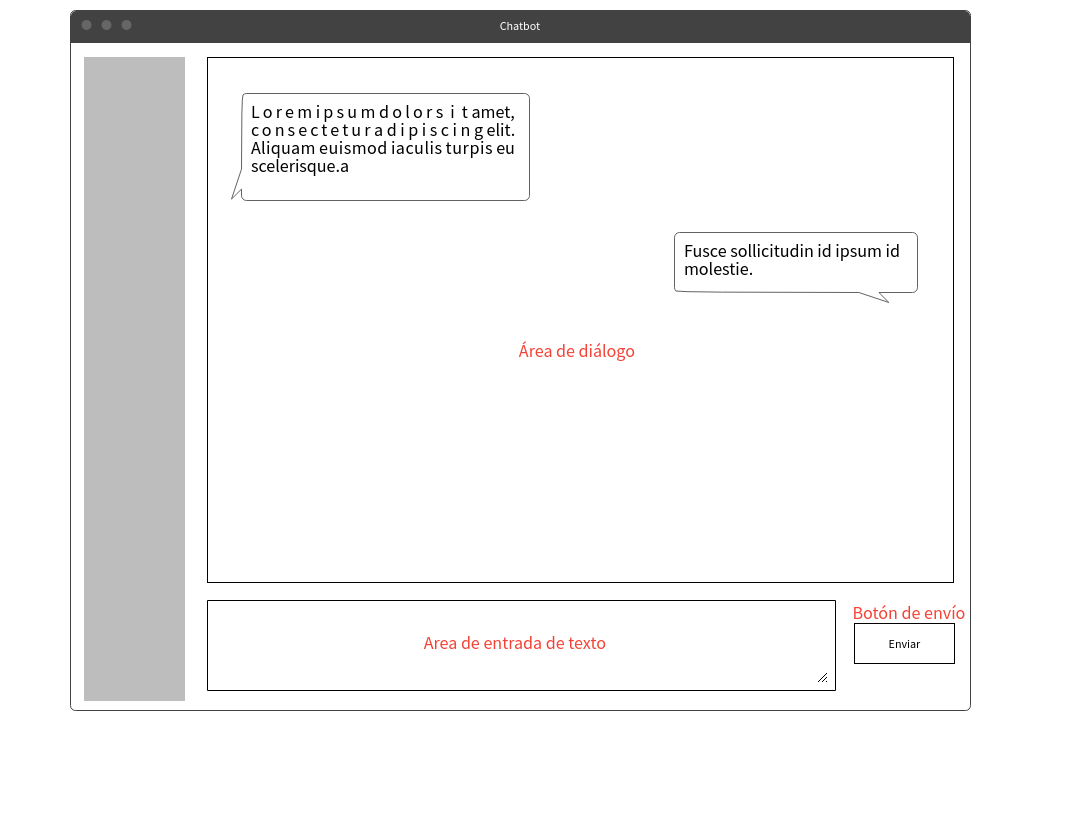
\includegraphics[scale=0.425]{images/5/interfaz-usuario}
    \caption{Diseño de la ventana de la interfaz de usuario mediante un navegador web.}
    \label{fig:interfaz-usuario}
\end{figure}

% \subsection{Diseño de la conversación}
% \label{sec:diseno-conversacion}

% \begin{figure}[ht]
%     \centering

%     \begin{tabular}{ | m{10em} | m{10em} |m{10em} | }
%         \hline
%         \textbf{Intención} & \textbf{Entidades} & \textbf{Acciones}\\
%         \hline
%         Saludar & - & Responder saludo \\
%         \hline
%         Solicitar reglamento & \textbf{titulo}, \textbf{capitulo}, \textbf{seccion}, \textbf{articulo} & Responder con reglamento\\
%         \hline
%         Buscar Conceptos & oración & Buscar artículos con conceptos similares \\
%         \hline
%         Despedir & - & Despedir al usuario \\
%         \hline
%     \end{tabular}
%     \caption{Tabla de relación entre intenciones y entidades.}
%     \label{fig:tabla-intenciones}
% \end{figure}

% \subsection{Intenciones}

% De acuerdo al requisito funcional \ref{itm:requisito-intenciones}, las intenciones que debe reconocer el chatbot son las siguientes:

% \begin{enumerate}
%     \item \textbf{Saludar}: Sirve como una formalidad por parte del bot saludando al usuario de acuerdo a la hora del día y que informa al usuario sobre la funcionalidad que puede hacer. Aunque siempre es iniciado cuando el usuario entra a la conversación, el usuario puede volver a saludar y el bot debe volver a responder.
%     \item Solicitar reglamento
%     \item Buscar conceptos
%     \item Despedir
% \end{enumerate}

% \subsection{Entidades}

% \begin{itemize}
%     \item 
% \end{itemize}
